\subsection{Charmonium acceptance and efficiency}\label{sec:Charmonia_Analysis_Efficiency}

This section presents the standard procedure used to estimate the charmonium acceptance and efficiency based on simulations. In order to improve the modelling of the \pt and rapidity spectra of charmonia, the kinematic distribution of the simulated dimuons are weighed as explained in \sect{sec:Charmonia_Analysis_Efficiency_JPsiCorr}. Afterwards, the \JPsi meson acceptance and efficiency are  determined from simulations as described in \sect{sec:Charmonia_Analysis_Efficiency_JPsiAcceptance} and \sect{sec:Charmonia_Analysis_Efficiency_JPsiEfficiency}, respectively. Then, the \JPsi meson efficiency is corrected using data-to-simulation efficiency ratios derived with the tag-and-probe method as detailed in \sect{sec:Charmonia_Analysis_Efficiency_JPsiCorrectedEfficiency}. Finally, the double ratio of prompt \PsiP over \JPsi meson efficiencies in \RunPbPb relative to \Runpp collisions are checked to be consistent with unity in \sect{sec:Charmonia_Analysis_Efficiency_Psi2SOverJPsiEfficiency}.


\subsubsection{Correction for charmonium \pt and rapidity}\label{sec:Charmonia_Analysis_Efficiency_JPsiCorr}

The detector acceptance and efficiency depends on the \pt and rapidity distributions of the detected particles. In order to derive reliable estimations from charmonium simulations, it is important to ensure that the kinematic distributions of charmonia are as close as possible to that of real data.

To accomplish this, a weight is assigned to each simulated dimuon according to their \rapMuMu and \ptMuMu. This weight is obtained from the ratio of the \JPsi-meson \pt spectrum measured in data over the one derived from simulation, in the different rapidity regions used in the \JPsi-meson analysis. The number of observed prompt and nonprompt \JPsi mesons extracted from the 2D fits to the \mMuMu and \ctau distributions in data, described in \sect{sec:Charmonia_Analysis_JPsiYieldExtraction}, are compared to the corresponding ones measured in the prompt and nonprompt \JPsiToMuMu simulations, respectively. The \ptMuMu distributions in each rapidity region are normalised to the number of observed  \JPsi mesons (prompt or nonprompt) in the inclusive region ($|\rapMuMu| < 2.4$ and $ 3.0 < \ptMuMu < 50$~\GeVc). The \JPsi-meson kinematic weights are then defined as:

\begin{equation}
 w^{\JPsi}\left(\ptMuMu, \rapMuMu\right) = \frac{\frac{1}{N^{\mu\mu}_{\text{data}}}\frac{\dd^{2}{N^{\mu\mu}_{\text{data}}}}{\dd{\ptMuMu}\dd{\rapMuMu}}\left(\ptMuMu, \rapMuMu\right)}{\frac{1}{N^{\mu\mu}_{\text{MC}}}\frac{\dd^{2}{N^{\mu\mu}_{\text{MC}}}}{\dd{\ptMuMu}\dd{\rapMuMu}}\left(\ptMuMu, \rapMuMu\right)}
\end{equation}

where $N^{\mu\mu}_{\text{data}}$ and $N^{\mu\mu}_{\text{MC}}$ are the number of \JPsi mesons measured in the inclusive region in data and simulation, respectively. The \JPsi-meson kinematic weights determined as a function of \ptMuMu, in the mid-rapidity region, are presented in \fig{fig:JPsiWeights}. They are found to vary between 0.4 and 1.6 depending on \ptMuMu and \rapMuMu.

\begin{figure}[htb!]
 \centering
 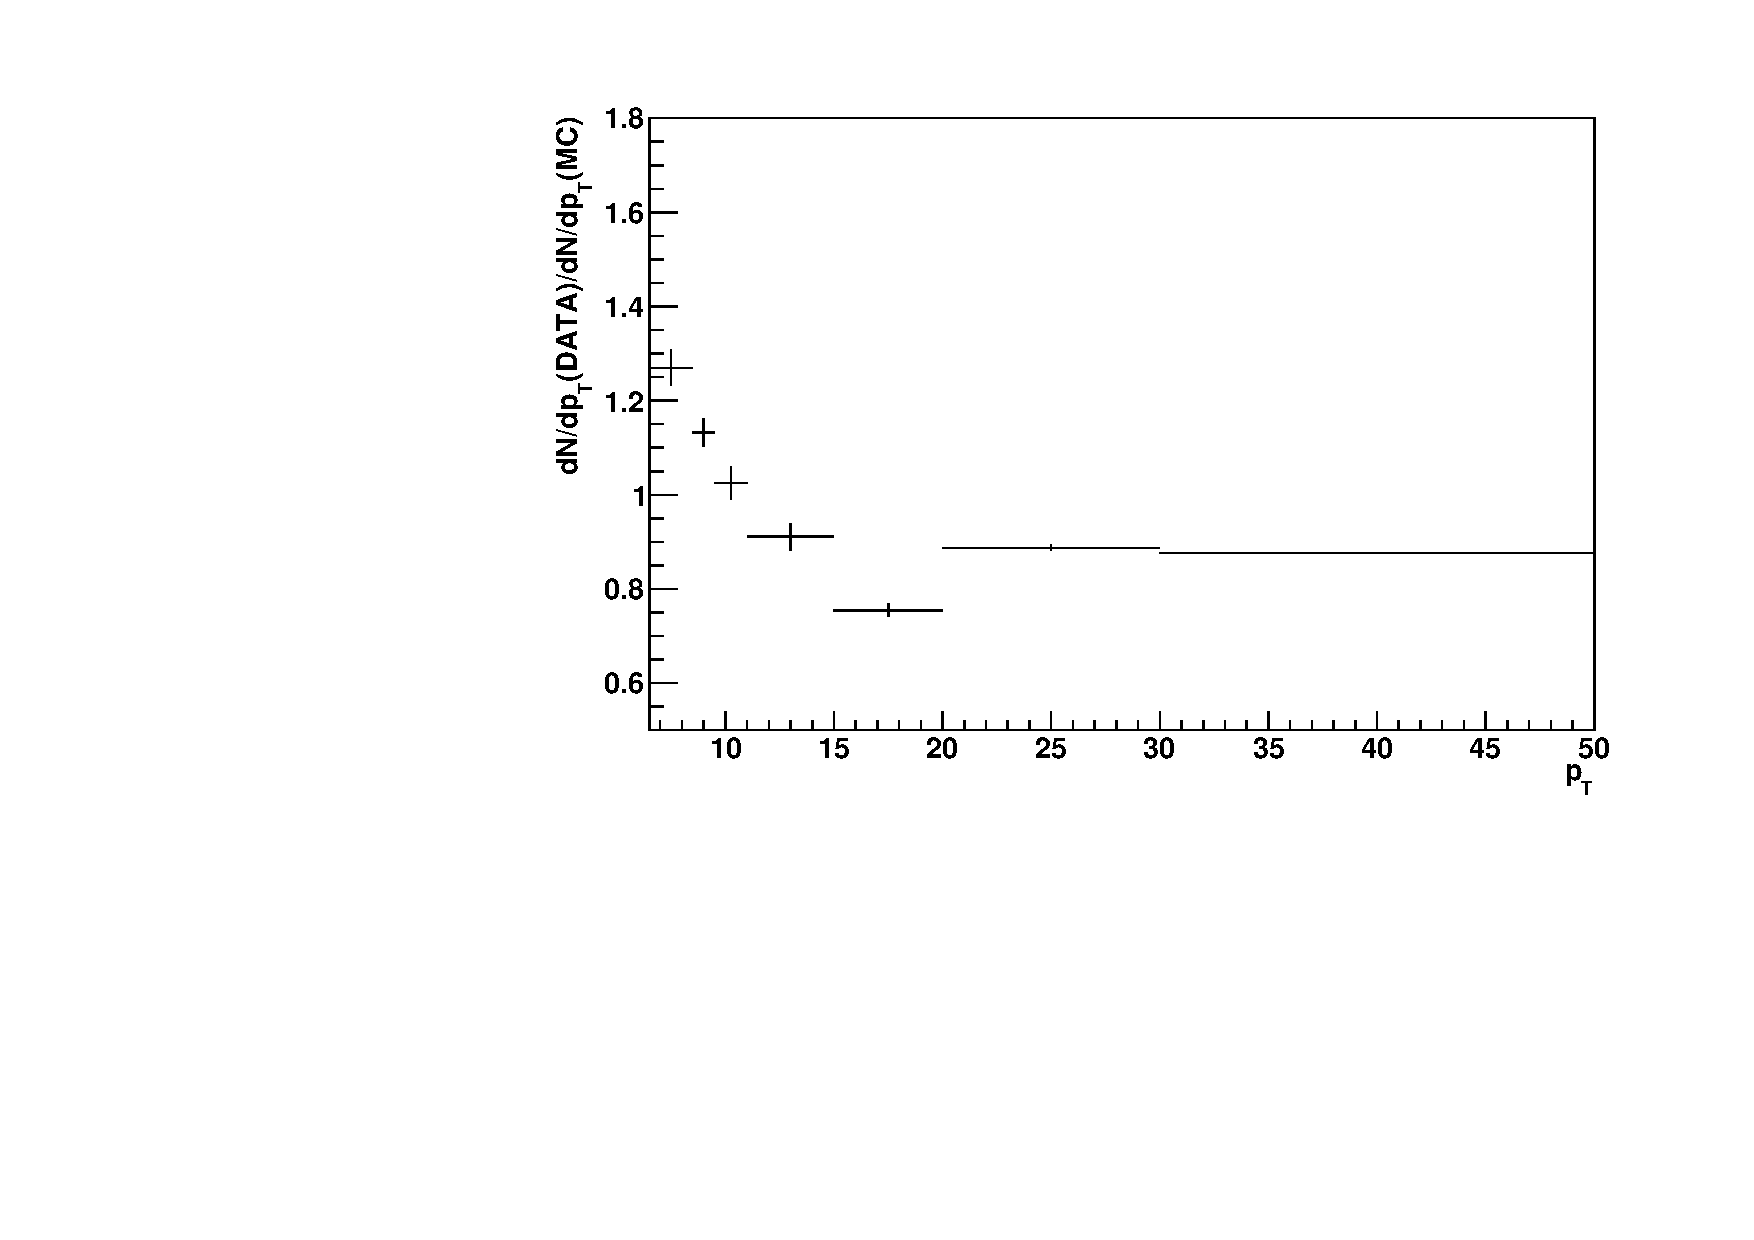
\includegraphics[width=0.48\textwidth]{Figures/Charmonia/Analysis/SignalEfficiency/JPsiWeights/PbPb_P_006.pdf}
 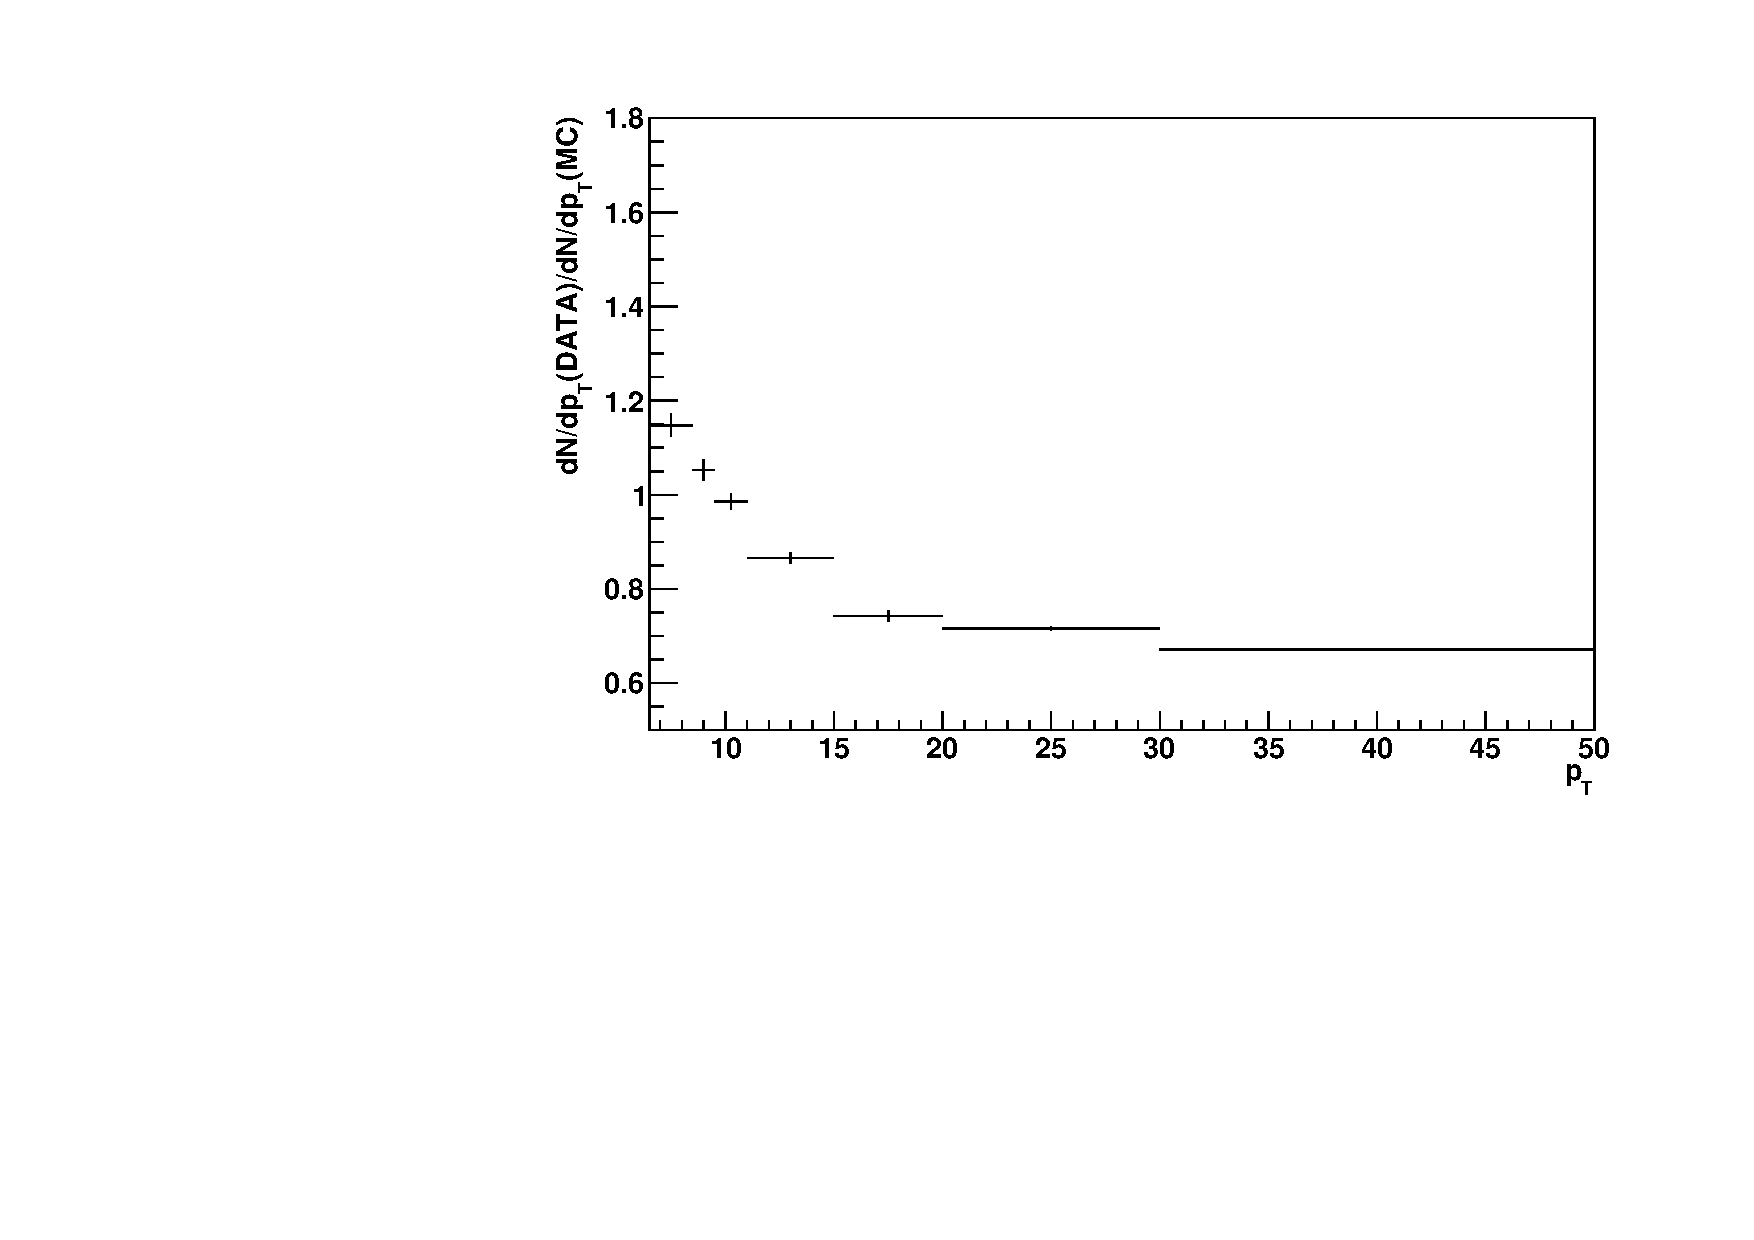
\includegraphics[width=0.48\textwidth]{Figures/Charmonia/Analysis/SignalEfficiency/JPsiWeights/PP_P_006.pdf}
 \caption{Data-to-simulation ratios of the prompt \JPsi-meson \pt distribution measured in the $|\rapMuMu| < 0.6$ rapidity region, in \RunPbPb (left) and \Runpp (right) collisions.}
 \label{fig:JPsiWeights}
\end{figure}

\subsubsection{Acceptance of \texorpdfstring{\JPsi}{J/psi} mesons}\label{sec:Charmonia_Analysis_Efficiency_JPsiAcceptance}

The \JPsi-meson acceptance is estimated using the \Runpp simulations. It is defined as the fraction of generated \mumu pairs from \JPsi-meson decays, with each muon satisfying the kinematic selection (labelled as \textit{in CMS}) listed in \sect{sec:Charmonia_Analysis_Selection_MuonKinematic}. The modelling of the \pt and rapidity of prompt and nonprompt \JPsi mesons is improved by weighing each generated dimuon, based on their \ptMuMu and \rapMuMu values, using the \JPsi-meson kinematic weights $w^{\JPsi}$ defined in the previous section. The \JPsi-meson acceptance ($\accJPsi$) is determined as a function of the generated dimuon \pt and rapidity, according to:

\begin{equation}
 \accJPsi\left(\ptMuMu , \rapMuMu\right) = \frac{N^{\JPsiToMuMu}_{\gen, \text{\PGm in CMS}} \left(\ptMuMu , \rapMuMu\right)}{N^{\JPsiToMuMu}_{\gen}\left(\ptMuMu , \rapMuMu\right)}
 \label{eq:JPsiMCAcceptance}
\end{equation}

where $N^{\JPsiToMuMu}_{\text{gen}}\left(\ptMuMu , \rapMuMu\right)$ is the number of generated dimuons in a given \ptMuMu and \rapMuMu range, and $N^{\JPsiToMuMu}_{\gen, \text{\PGm in CMS}}\left(\ptMuMu , \rapMuMu\right)$ represents the number of those satisfying the muon kinematic selection.

The \JPsi-meson acceptance derived from the prompt \JPsi simulations is presented in \fig{fig:JPsiAcc_pp}. The trend observed as a function of dimuon \pt and rapidity is caused by the CMS muon kinematic coverage. \JPsi mesons produced in the forward region or at higher \pt are more likely to decay to muons that reach the CMS muon stations than those produced at mid-rapidity or lower \pt.

\begin{figure}[htb!]
 \centering
 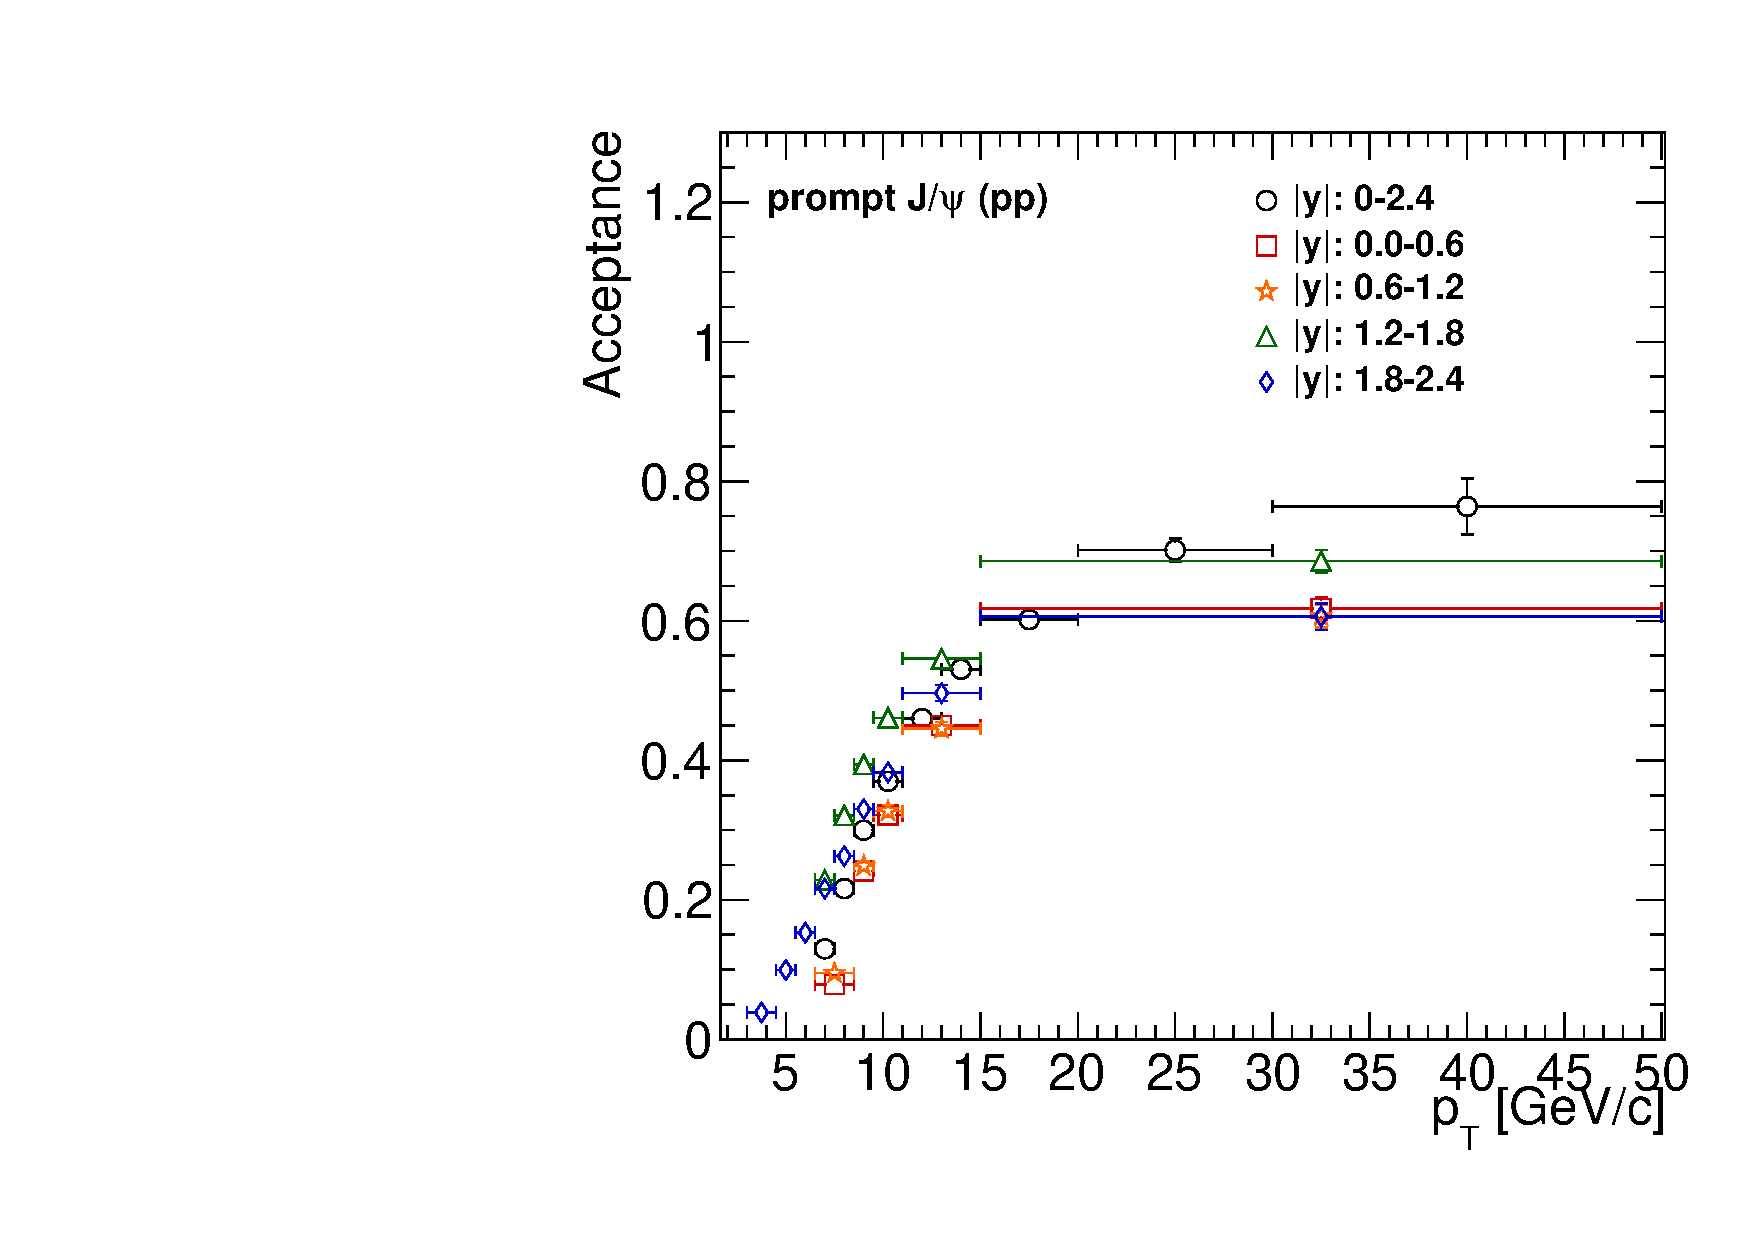
\includegraphics[width=0.45\textwidth]{Figures/Charmonia/Analysis/SignalEfficiency/Acceptance/jpsi_pp_pt_rap.pdf}
 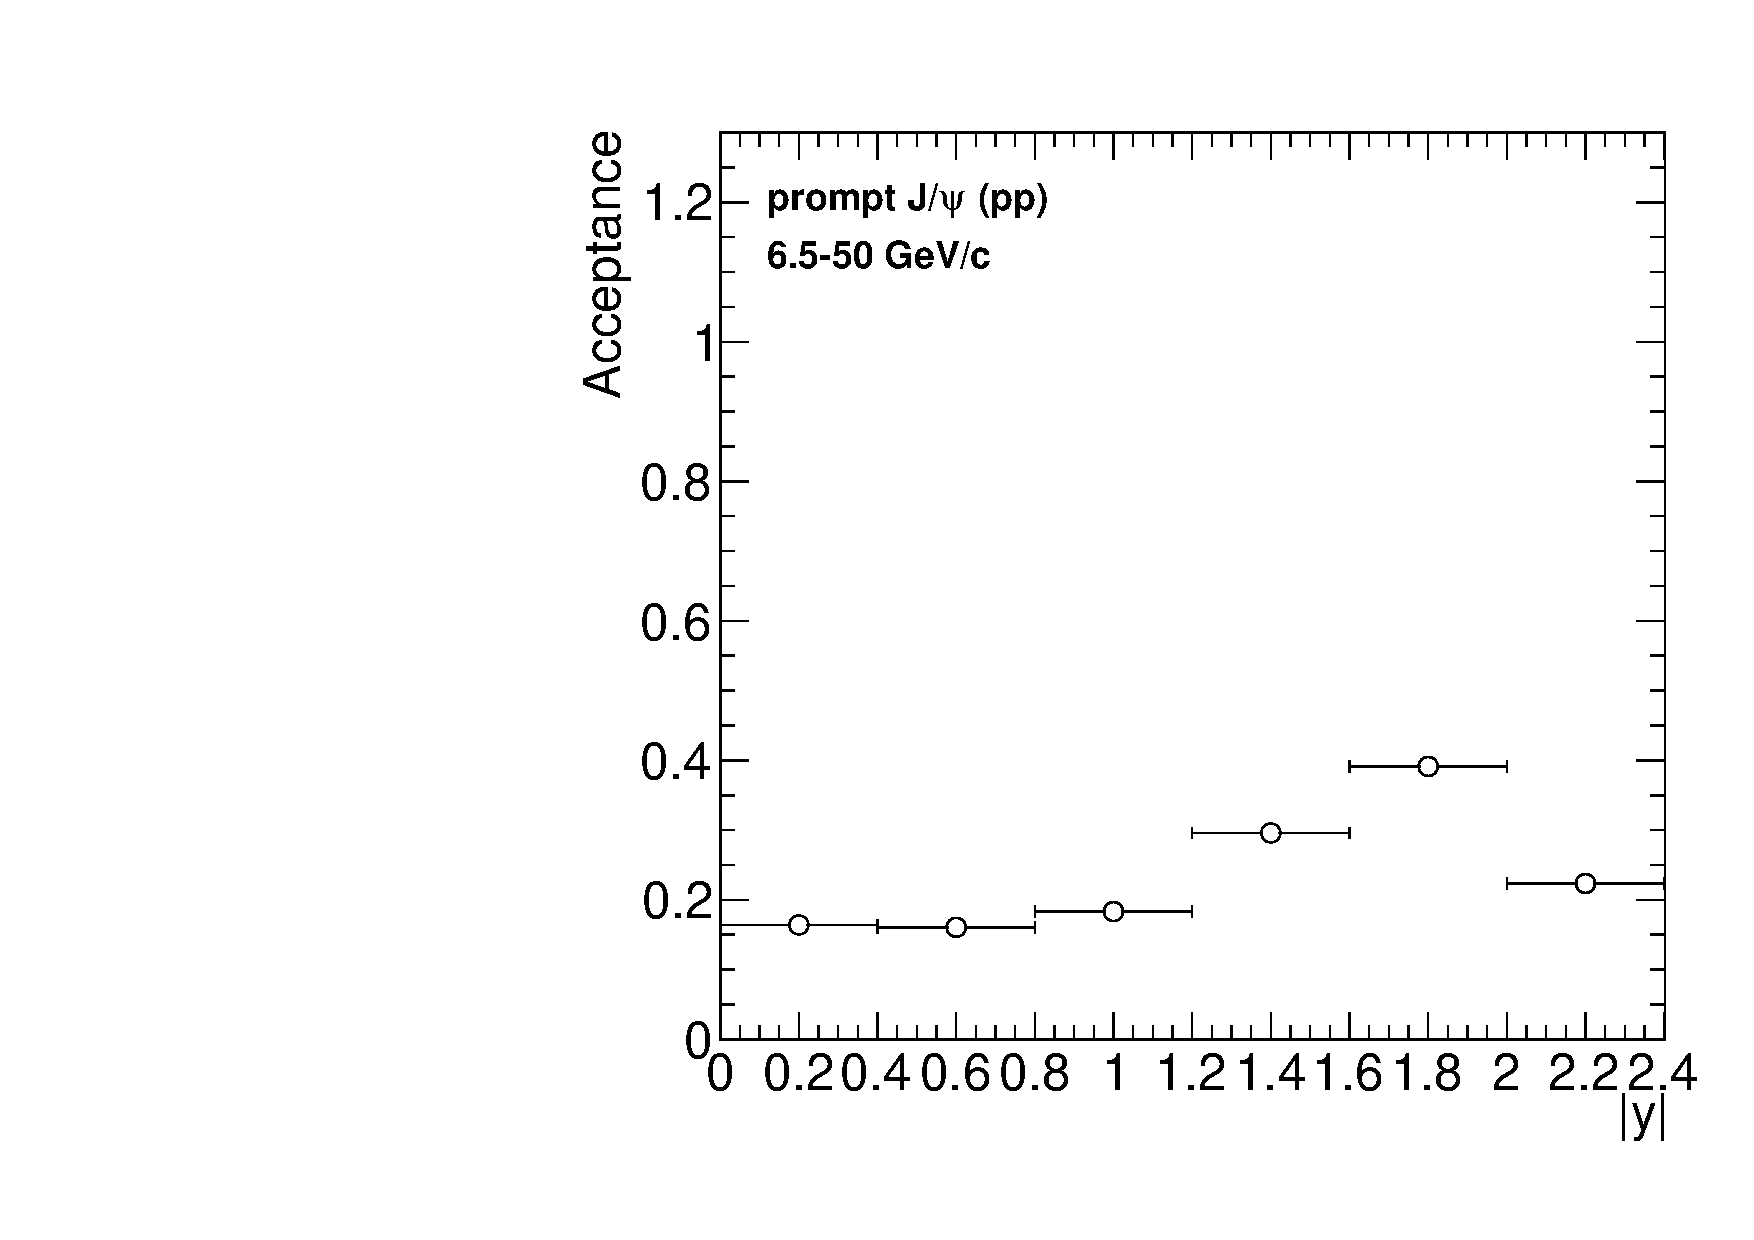
\includegraphics[width=0.45\textwidth]{Figures/Charmonia/Analysis/SignalEfficiency/Acceptance/jpsi_pp_rap.pdf}
 \caption{Acceptance of prompt \JPsi mesons, estimated from simulations, as a function of \ptMuMu (left) and \rapMuMu (right). The error bars represents the statistical uncertainties.}
 \label{fig:JPsiAcc_pp}
\end{figure}

\subsubsection{Efficiency of \texorpdfstring{\JPsi}{J/psi} mesons}\label{sec:Charmonia_Analysis_Efficiency_JPsiEfficiency}

The \JPsiToMuMu simulations are used to measure the efficiency of prompt and nonprompt \JPsi mesons, in \Runpp and \RunPbPb collisions. In this case, a reconstructed \mumu pair is considered to be an offline dimuon if it satisfies the charmonium selection requirements detailed in Sections  \ref{sec:Charmonia_Analysis_Selection_MuonIdentification} to  \ref{sec:Charmonia_Analysis_Selection_CharmoniumSelection}. Among these selection criteria, each reconstructed muon is required to satisfy the muon kinematic selection and identification criteria, and match the trigger. Also, the two muon tracks of the offline dimuon are required to derive from a common vertex with $\chi^{2}$ probability larger than 1\%. 

The \JPsi-meson efficiency is defined as the fraction of generated \mumu pairs in the acceptance that can be matched to an offline dimuon, with each generated muon satisfying the kinematic selection. The matching between a generated and an offline \mumu pair is performed by requiring that each generated and reconstructed muon of same charge are within $\Delta{R}(\mu_{\mathrm{gen}},\mu_{\mathrm{reco}}) < 0.03$. The \pt and rapidity spectra of  the offline and generated dimuons are weighed per event with the $w^{\JPsi}$ kinematic weights, as was done in the previous section. The \JPsi-meson efficiency ($\effJPsi$) is computed as a function of the dimuon \pt and rapidity, according to:

\begin{equation}
 \effJPsi\left(\ptMuMu , \rapMuMu\right) = \frac{N^{\JPsiToMuMu}_{\text{offline}}\left(\ptMuMu , \rapMuMu\right)}{N^{\JPsiToMuMu}_{\gen, \text{\PGm in CMS}} \left(\ptMuMu , \rapMuMu\right)}
 \label{eq:JPsiMCEfficiency}
\end{equation}

where $N^{\JPsiToMuMu}_{\text{offline}}$ and $N^{\JPsiToMuMu}_{\gen, \text{\PGm in CMS}}$ are the number of offline and generated pairs of muons within the kinematic acceptance of the analysis, accordingly.

\subsubsection{Efficiency of \texorpdfstring{\JPsi}{J/psi} mesons corrected with the tag-and-probe method}\label{sec:Charmonia_Analysis_Efficiency_JPsiCorrectedEfficiency}

In order to take into account possible discrepancies between the muon efficiencies in simulation and those in data, the \JPsi-meson efficiencies are corrected with a set of data-to-simulation corrections provided by the CMS HIN group and derived using the tag-and-probe method. This collective work, to which I only participated marginally, is documented in an internal analysis note~\cite{Muon_TnP_PbPb}.

The \tnp corrections for \RunPbPb and \Runpp efficiencies are computed following a procedure similar to the one used for \RunpPb collisions, which is described in detail in \sect{sec:WBoson_Analysis_Efficiency_Corrected}. The main difference is that it addresses lower muon momentum. To provide these muons, a sample of \JPsi mesons is used instead of \Z bosons. Thus, the \tnp corrections are extracted from the prompt \JPsiToMuMu simulations and from a data sample of single muon events selected with the HLT trigger. The \tnp method is used to measure the standalone-muon reconstruction, tracking, identification and trigger efficiencies in data and simulation. Apart from the different muon identification and trigger criteria, these \tnp efficiencies are probed in the same way as done for \RunpPb collisions. The \tnp efficiencies are extracted by fitting the tag-probe invariant mass distribution, within the \JPsi mass region ($2.6 < \mMuMu < 3.5$~\GeVcc), for probes passing and failing the criteria of each efficiency under study.

After comparing the \tnp efficiencies extracted from data and simulation, it is found that the muon simulated efficiencies for standalone-muon reconstruction, tracking and identification, are in good agreement with the data efficiencies. However, the trigger efficiencies are observed to disagree between simulation and data both in \Runpp and \RunPbPb collisions, as shown in \fig{fig:TnPJpsi}. As a result, only the simulated trigger efficiency requires a correction.

\begin{figure}[htb!]
 \centering
 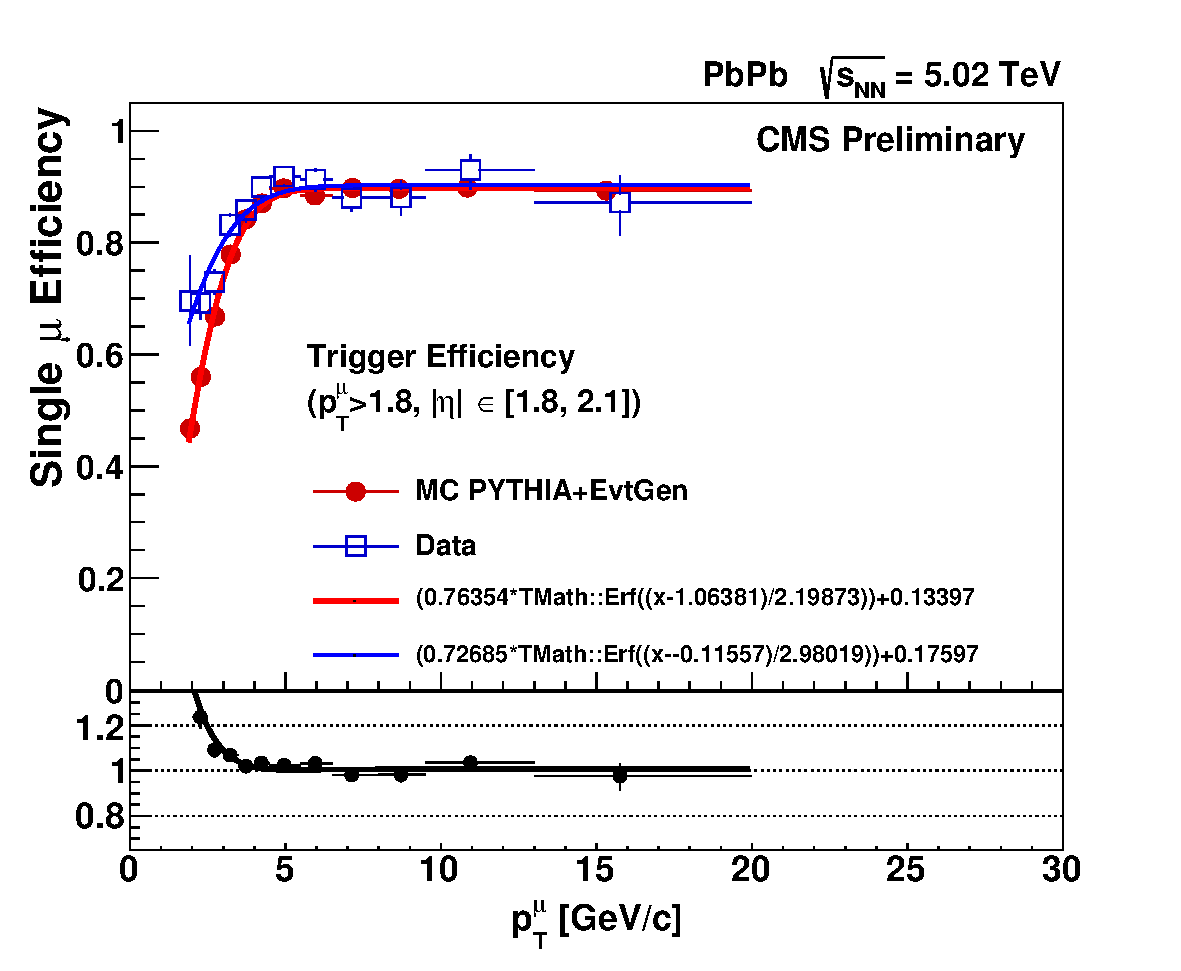
\includegraphics[width=0.45\textwidth]{Figures/Charmonia/Analysis/SignalEfficiency/TnP/tpTreeSF2_PbPb_RD_MC_PT.pdf}
 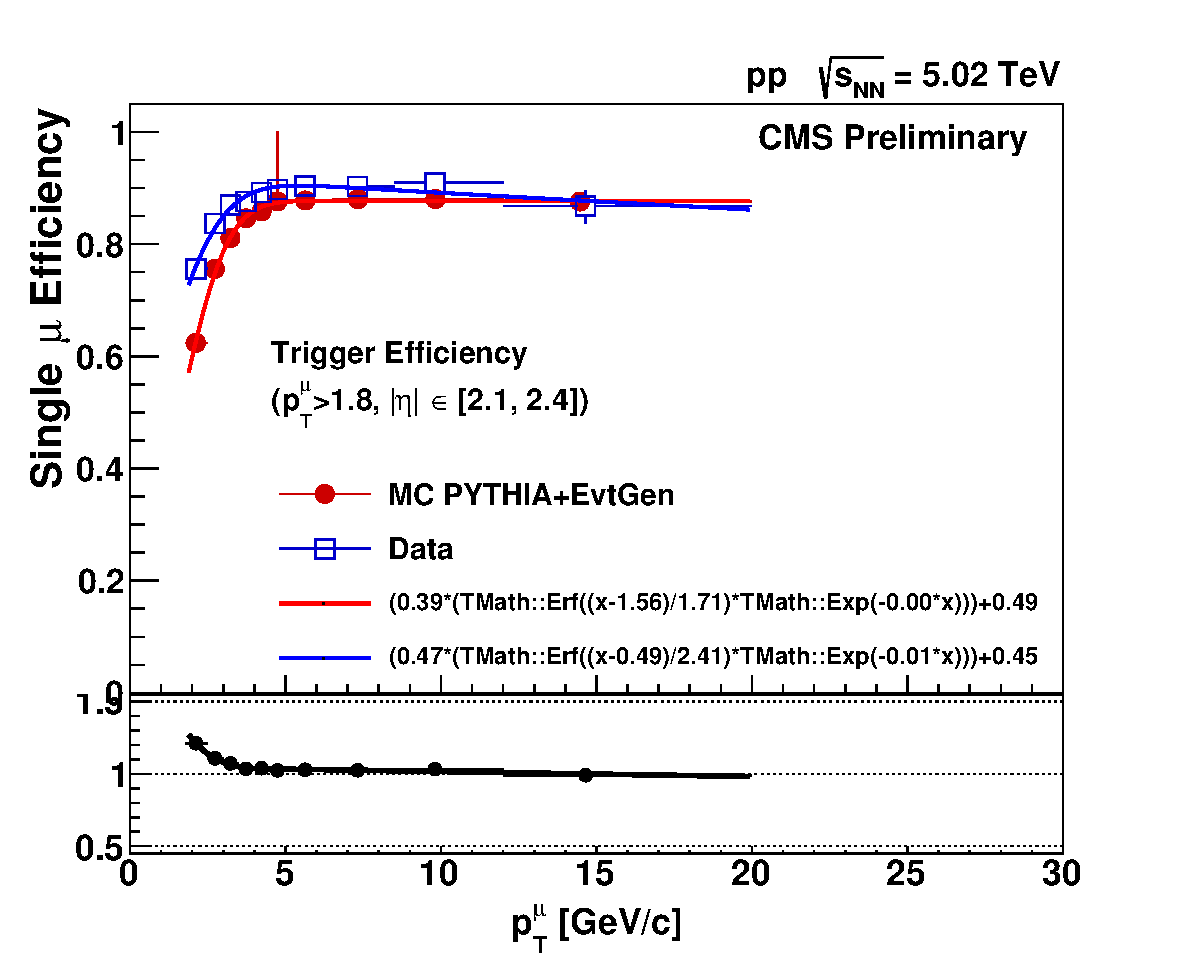
\includegraphics[width=0.45\textwidth]{Figures/Charmonia/Analysis/SignalEfficiency/TnP/tpTreeSF3_pp_RD_MC_PT.pdf}
 \caption{Muon trigger efficiencies as a function of the probe \pt. The efficiencies are extracted, using the \tnp method, from data (blue) and simulation (red) in \RunPbPb collisions at $1.8<|\etaMu|<2.1$ (left) and \Runpp collisions at $2.1<|\etaMu|<2.4$ (right). The bottom panels show the data-to-simulation efficiency ratio. The results of the fits to the efficiencies are also shown. Figures taken from the private Ref.~\cite{Muon_TnP_PbPb}.}
 \label{fig:TnPJpsi}
\end{figure}

The muon trigger efficiencies are measured with respect to the probe \pt, in four $|\eta|$ regions with boundaries: [0.0, 1.2, 1.8, 2.1, 2.4]. The \pt dependence in each $|\eta|$ region is parametrised with a function of the form $f_{\text{trig}}(\pt) = c_{1}\cdot\text{Erf}[(\pt - c_{2})/c_{3}]\cdot\exp[c_{4}\cdot\pt] + c_{5}$, where $\text{Erf}$ is the error function and $c_{i}$ are free parameters. The \tnp-correction weight for the trigger efficiency is then derived from the ratio of the fitted functions, extracted from data and simulation, as a function of probe \pt in each $|\eta|$ region, given by:

\begin{equation}
 w_{\text{trig}}\left(\pt, |\eta|\right) = \left[\frac{f^{\data}_{\text{trig}}\left(\pt\right)}{f^{\MC}_{\text{trig}}\left(\pt\right)}\right]\left({|\eta|}\right)
\end{equation}

To apply the \tnp corrections, the \JPsi-meson efficiency is recomputed by weighing each offline dimuon with the \tnp-correction weights for each muon to trigger, according to:

\begin{equation}
 \effJPsi = \frac{\left[\sum\limits_{i=1}^{N^{\JPsiToMuMu}_{\text{offline}}} w_{\text{trig}}\left(\pt^{\mu,{+}}, |{\eta^{\mu,{+}}}|\right) \cdot w_{\text{trig}}\left(\pt^{\mu,{-}}, |{\eta^{\mu,{-}}}|\right)\right]}{N^{\JPsiToMuMu}_{\gen, \text{\PGm in CMS}}}
\end{equation}

where $\pt^{\mu,{+}(\mu,{-})}$ is the transverse momentum of positive (negative) charged muons, and $\eta^{\mu,{+}(\mu,{-})}$ is the corresponding pseudorapidity. The \tnp corrections increase the \JPsi-meson efficiency by 35\% at $3 < \ptMuMu < 6.5$~\GeVc, while the range of variation at $\ptMuMu > 10$~\GeVc is less than 4\%. The corrected \JPsi-meson efficiencies are shown for \Runpp and \RunPbPb simulated events in \fig{fig:JPsiCorrEff_PP} and  \fig{fig:JPsiCorrEff_PbPb}, respectively.

\begin{figure}[htb!]
 \centering
 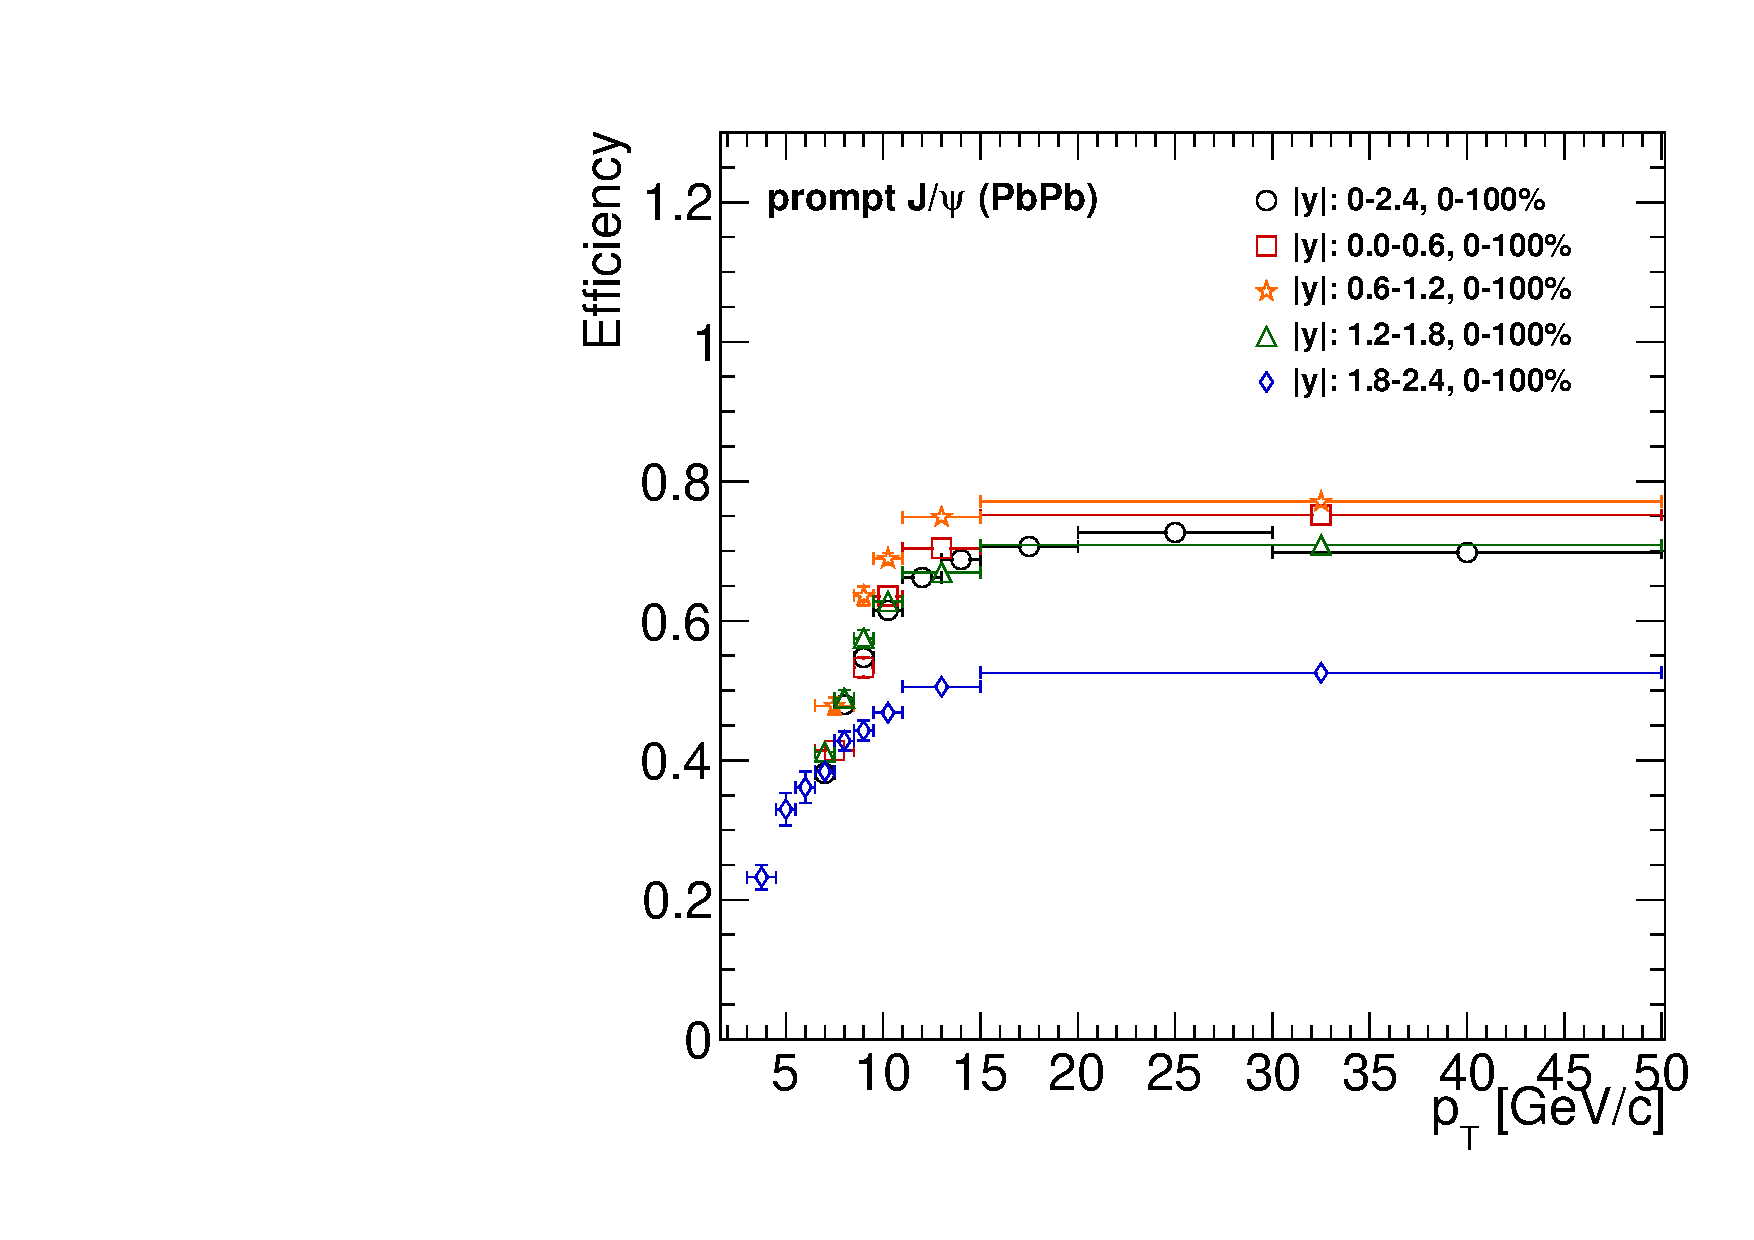
\includegraphics[width=0.45\textwidth]{Figures/Charmonia/Analysis/SignalEfficiency/Efficiency/jpsi_pbpb_pt_rap.pdf}
 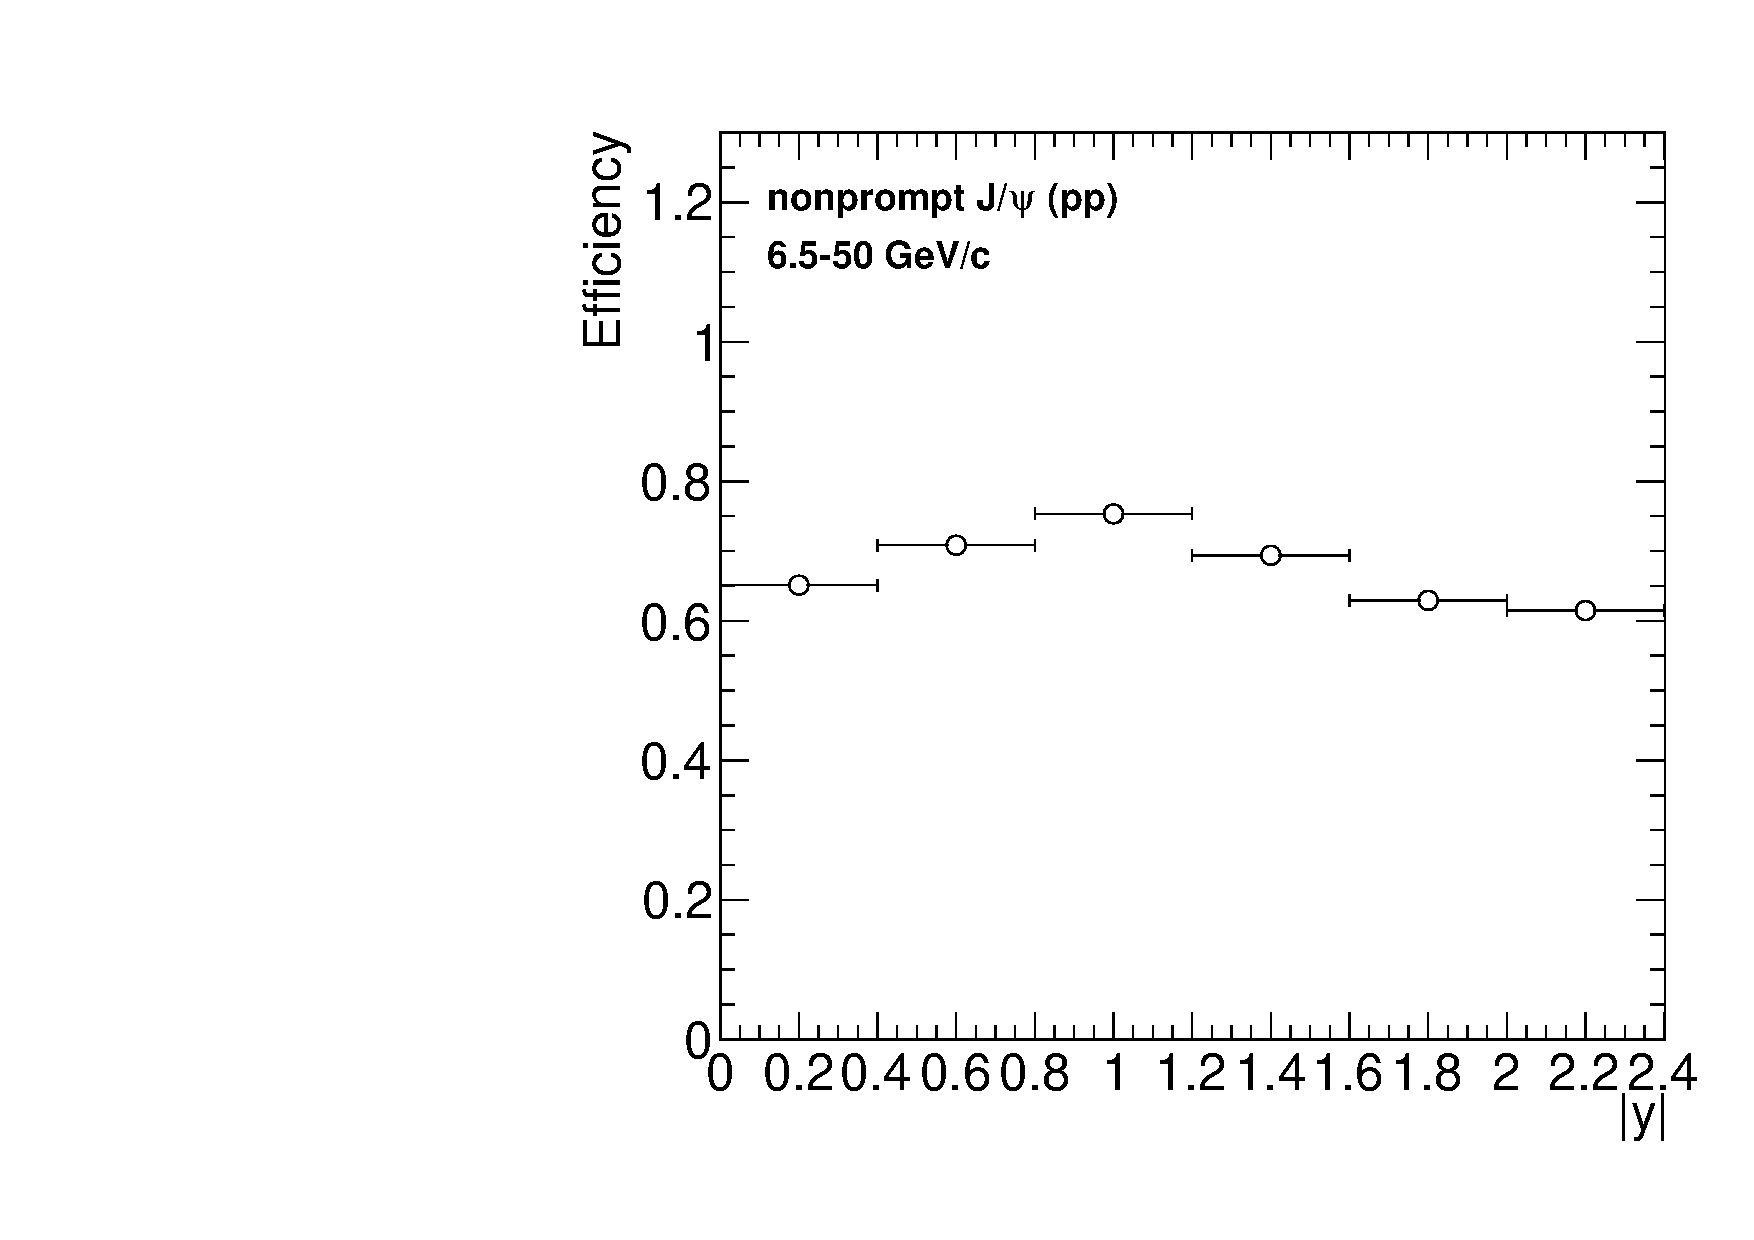
\includegraphics[width=0.45\textwidth]{Figures/Charmonia/Analysis/SignalEfficiency/Efficiency/npjpsi_pp_rap.pdf}
 \caption{Corrected efficiencies of prompt \JPsi mesons measured in \Runpp collisions, as a function of \ptMuMu (left) and rapidity (right) in different rapidity regions. The error bars represent statistical uncertainties.}
 \label{fig:JPsiCorrEff_PP}
\end{figure}

\begin{figure}[htb!]
 \centering
 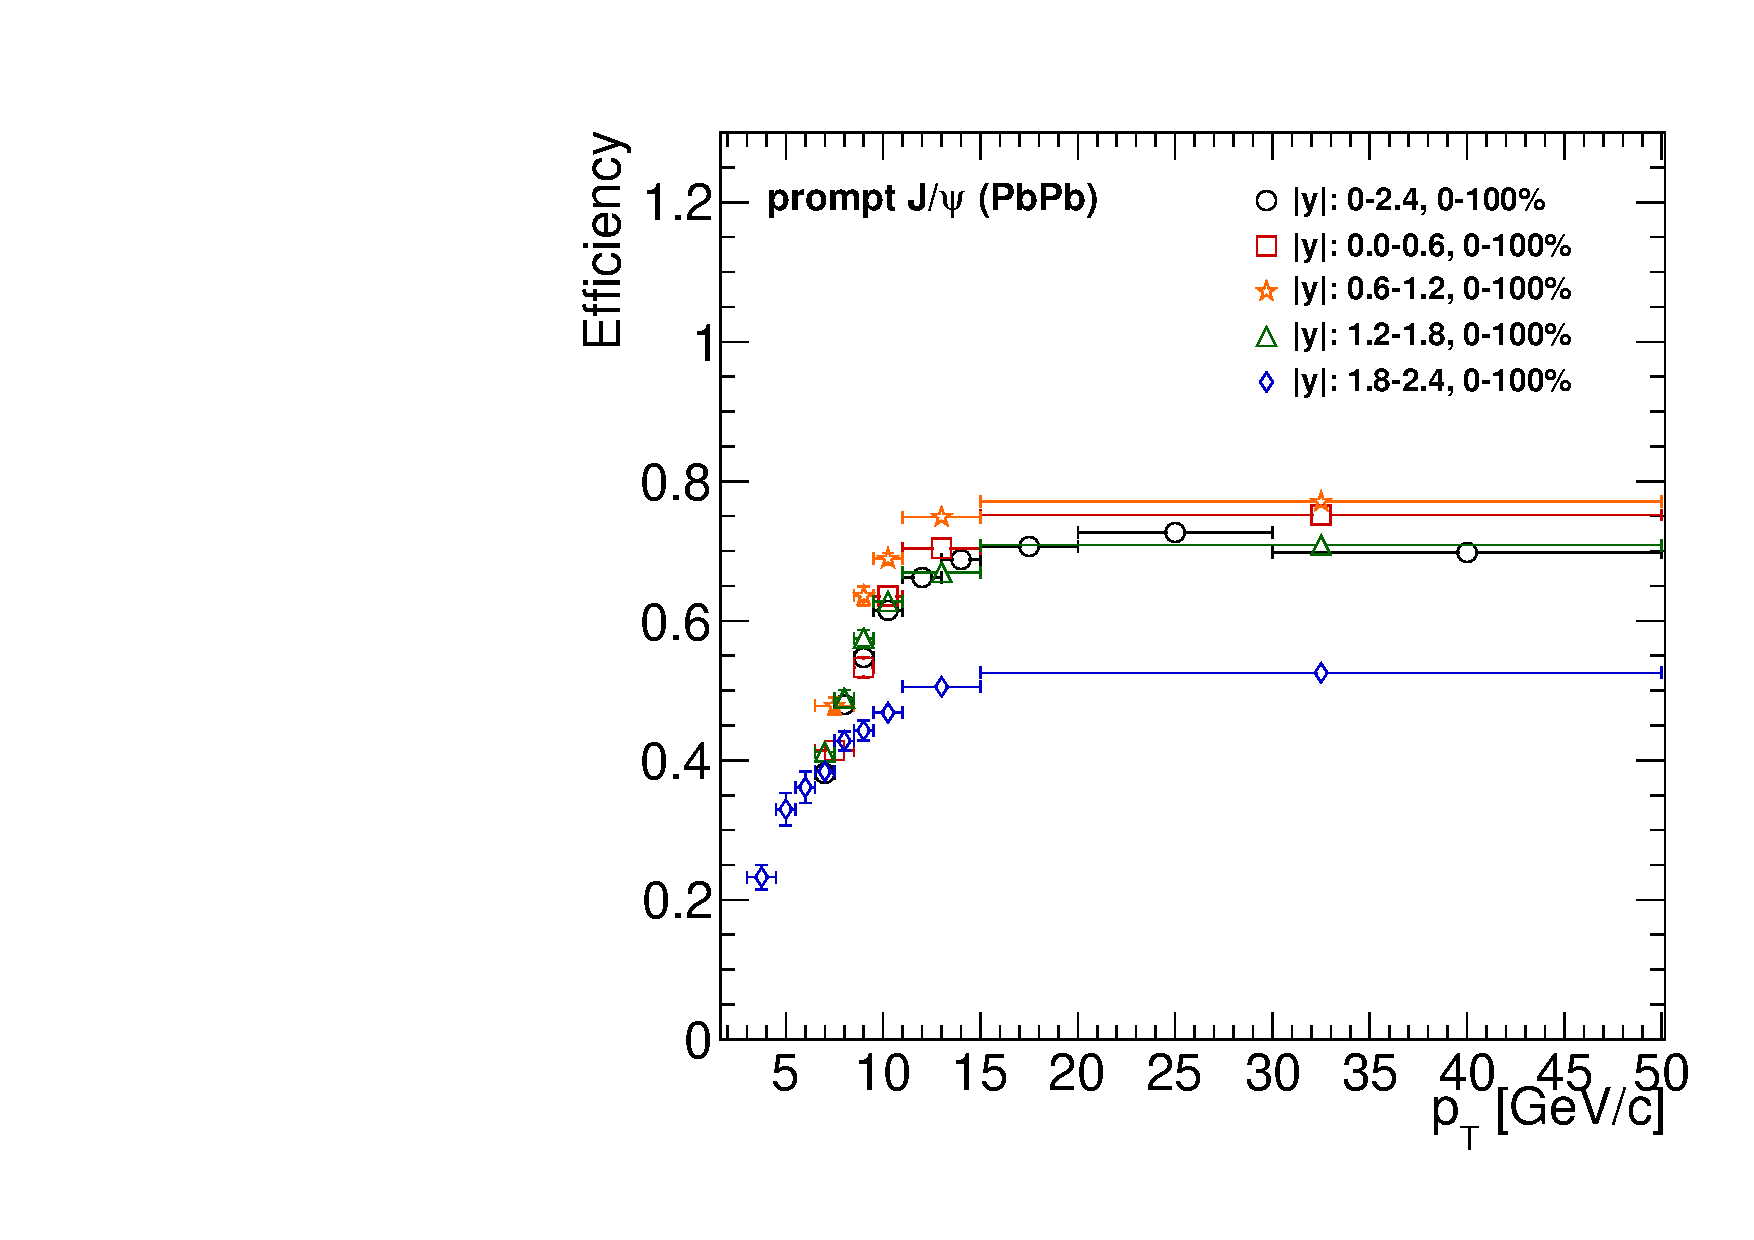
\includegraphics[width=0.45\textwidth]{Figures/Charmonia/Analysis/SignalEfficiency/Efficiency/jpsi_pbpb_pt_rap.pdf}
 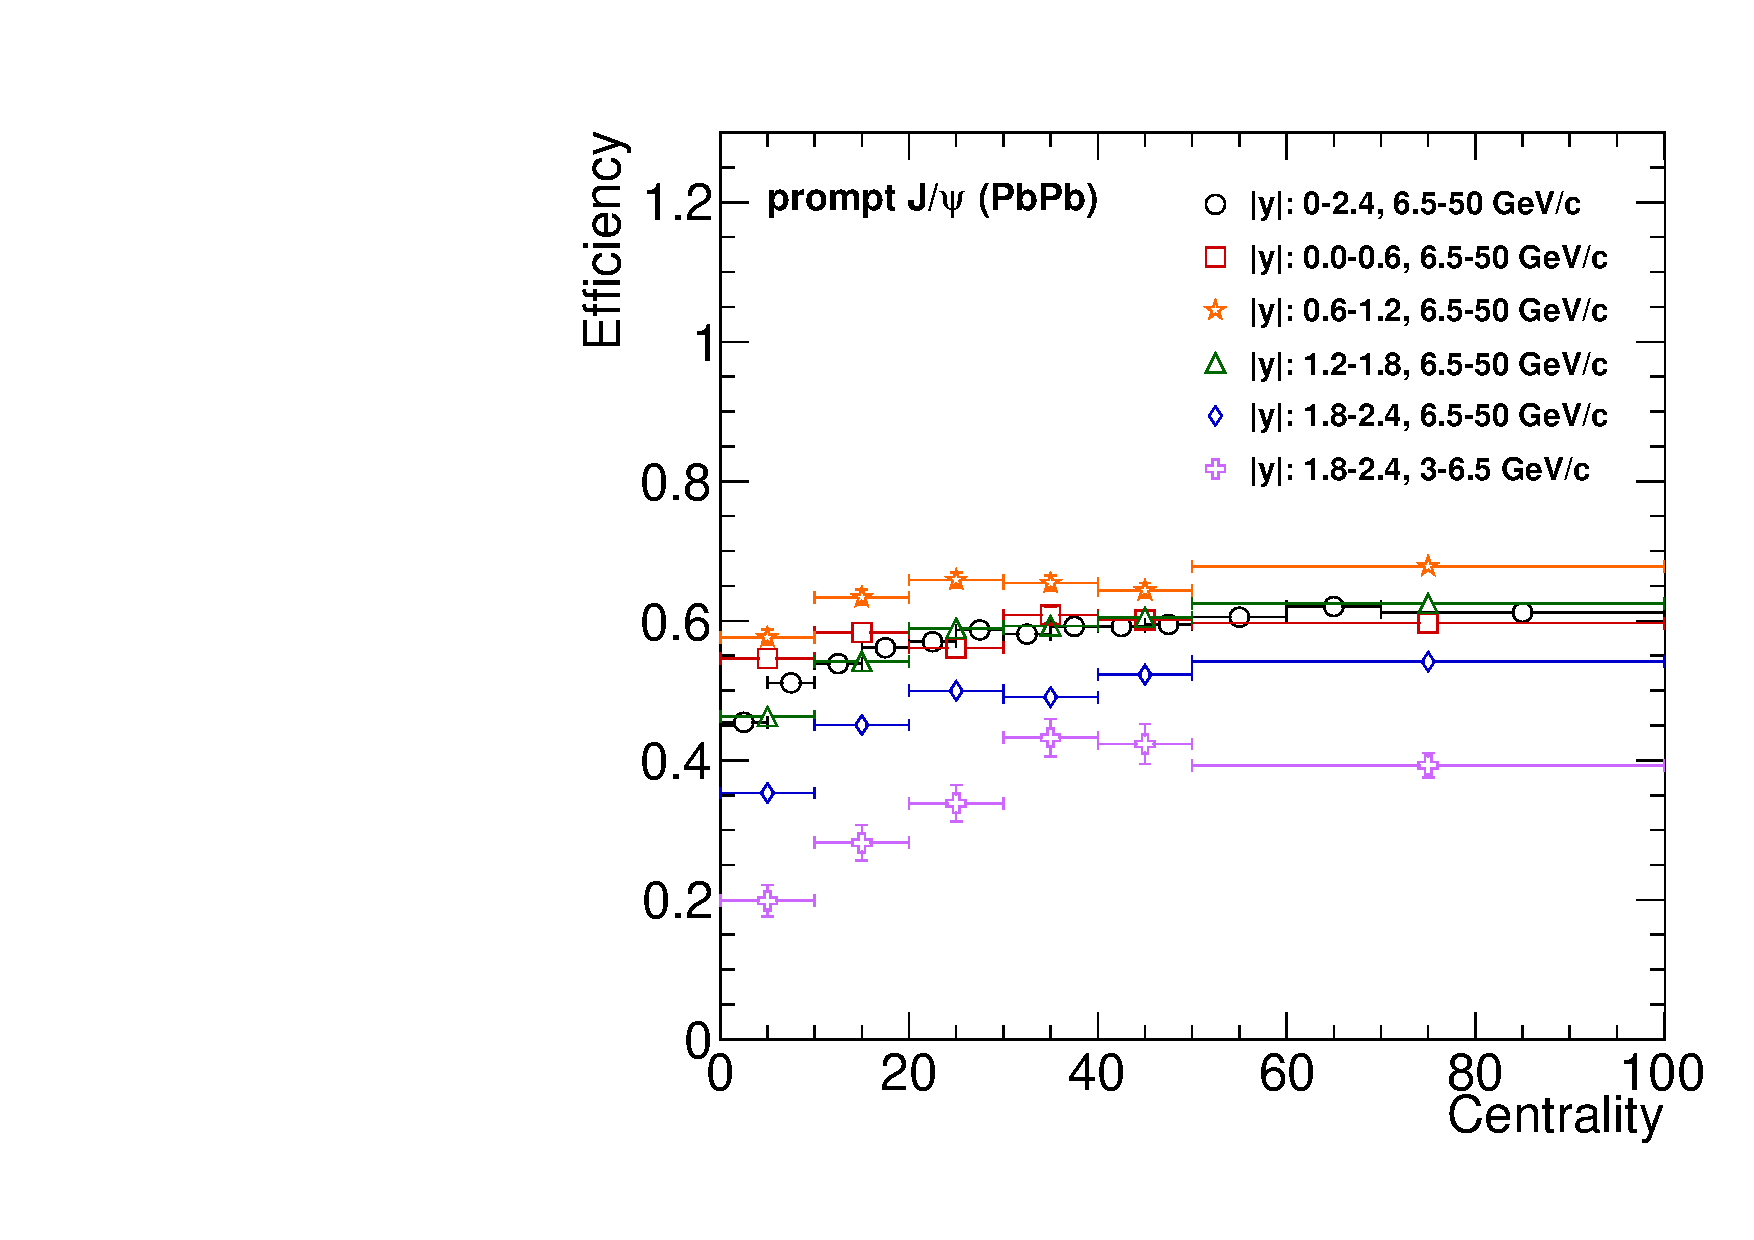
\includegraphics[width=0.45\textwidth]{Figures/Charmonia/Analysis/SignalEfficiency/Efficiency/jpsi_pbpb_cent_rap.pdf}
 \caption{Corrected efficiencies of prompt \JPsi mesons measured in \RunPbPb collisions, as a function of \ptMuMu (left) and centrality (right), in different rapidity regions. The error bars represent statistical uncertainties.}
 \label{fig:JPsiCorrEff_PbPb}
\end{figure}

\subsubsection{Double ratio of prompt \texorpdfstring{\PsiP}{psi(2S)}/\texorpdfstring{\JPsi}{J/psi} efficiencies}\label{sec:Charmonia_Analysis_Efficiency_Psi2SOverJPsiEfficiency}

Since the prompt \PsiP and \JPsi mesons have similar masses and production mechanisms, it is expected that their efficiencies cancel at first order when measuring the double ratio of prompt charmonium yields in \RunPbPb relative to \Runpp collisions. In order to check this, the efficiency of \PsiP mesons ($\effPsiP$) is estimated from the prompt \PsiPToMuMu simulation, following the same procedure used to determine the \JPsi meson efficiency, described in the previous sections.

The prompt \PsiP and \JPsi meson efficiencies are computed in \Runpp and \RunPbPb collisions, including the \ctau selection defined in \sect{sec:Charmonia_Analysis_PsiPoverJPsiRatioExtraction}, and the double ratio of prompt charmonium efficiencies is then computed as:

\begin{equation}
 \chi^{\PsiP/\JPsi} = \frac{\left(\effPsiP\biggr/\effJPsi\right)_{\PbPb}}{\left(\effPsiP\biggr/\effJPsi\right)_{\pp}}
\end{equation}

The results of the double ratio of prompt charmonium efficiencies are presented in \fig{fig:DoubleRatioEff}. It is observed that the $\chi^{\PsiP/\JPsi}$ is consistent with unity overall as expected. Thus, the measurements of the double ratio of prompt charmonium yields do not require to be  corrected for detector efficiency, and the difference with respect to unity is assigned as a systematic uncertainty as detailed in \sect{sec:Charmonia_Analysis_PsiPoverJPsiRatioSystematics_Effiency}.

\begin{figure}[htb!]
 \centering
 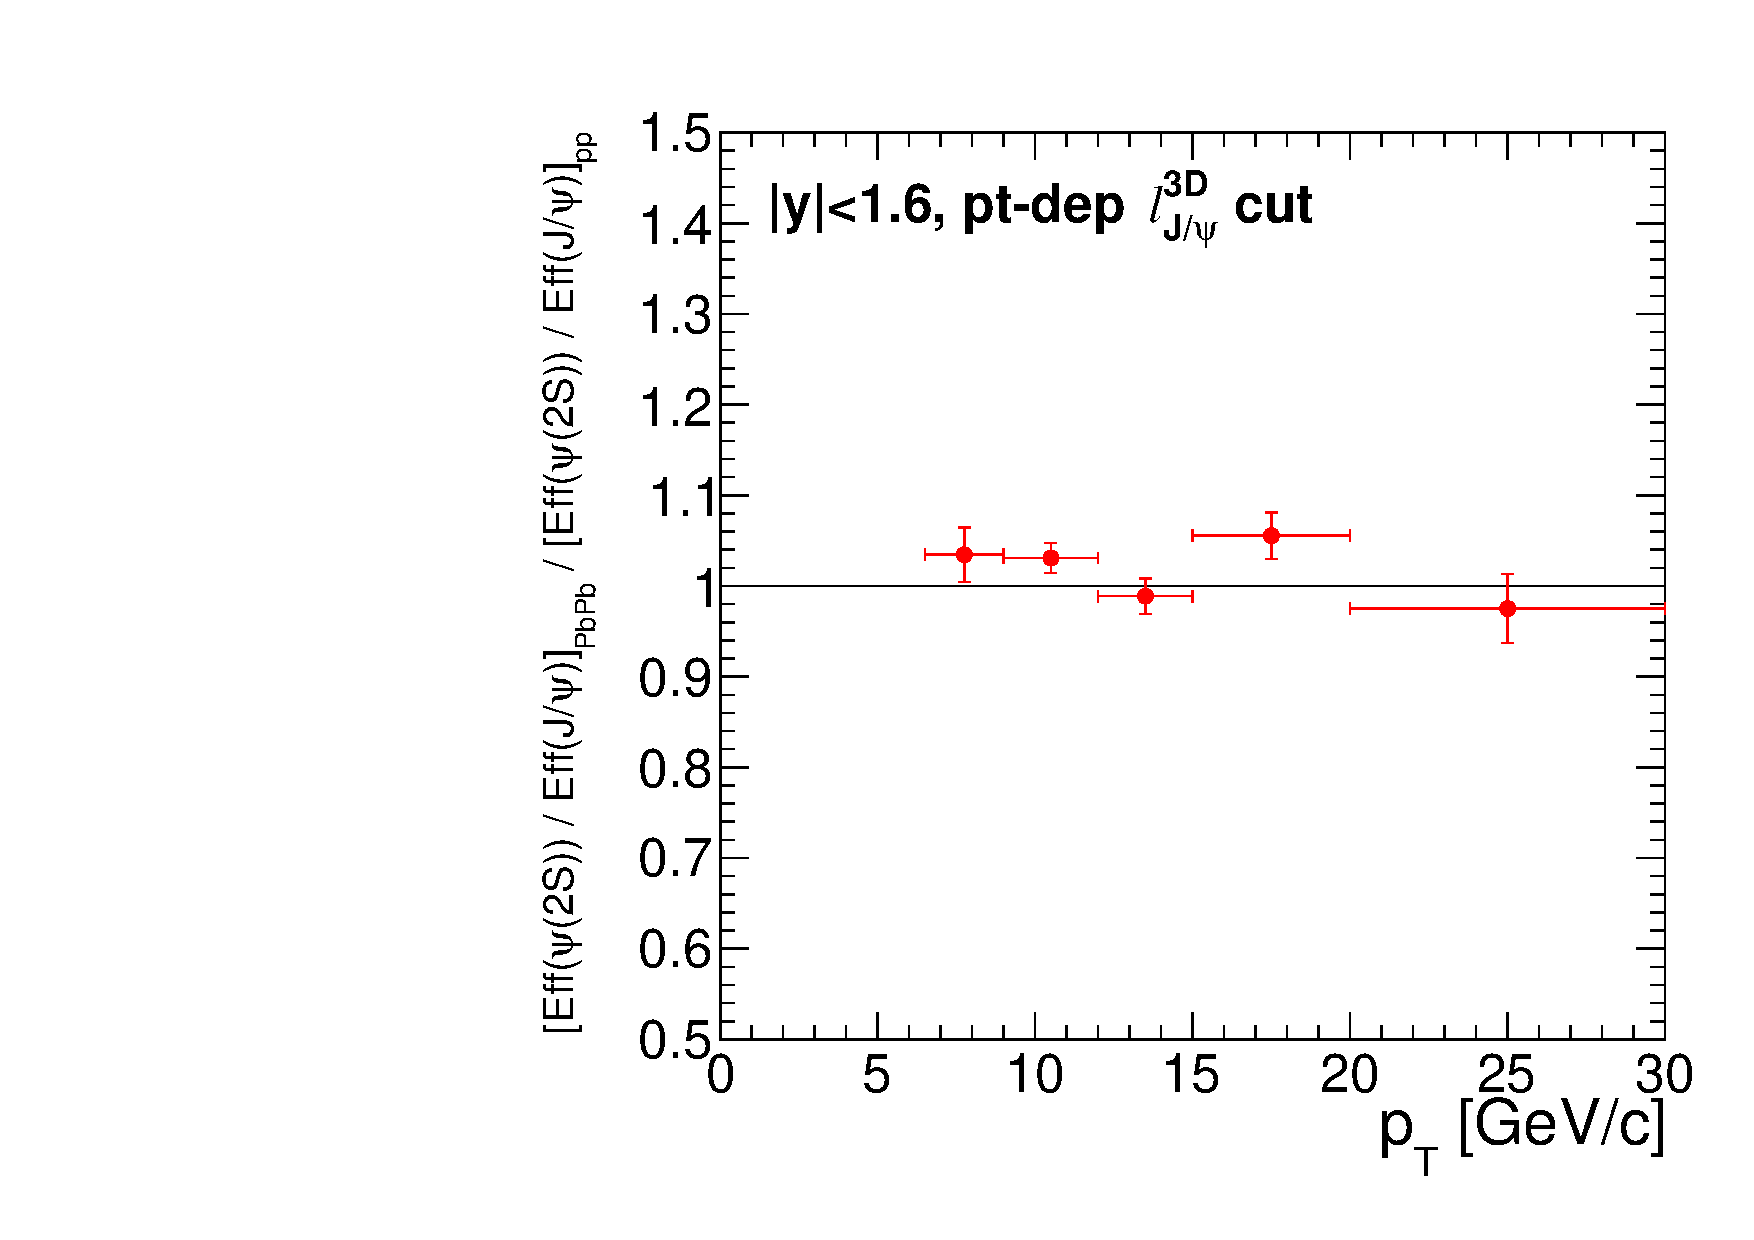
\includegraphics[width=0.45\textwidth]{Figures/Charmonia/Analysis/SignalEfficiency/DoubleRatio/doubleratio_pt_mid_ptdepcut_.pdf}
 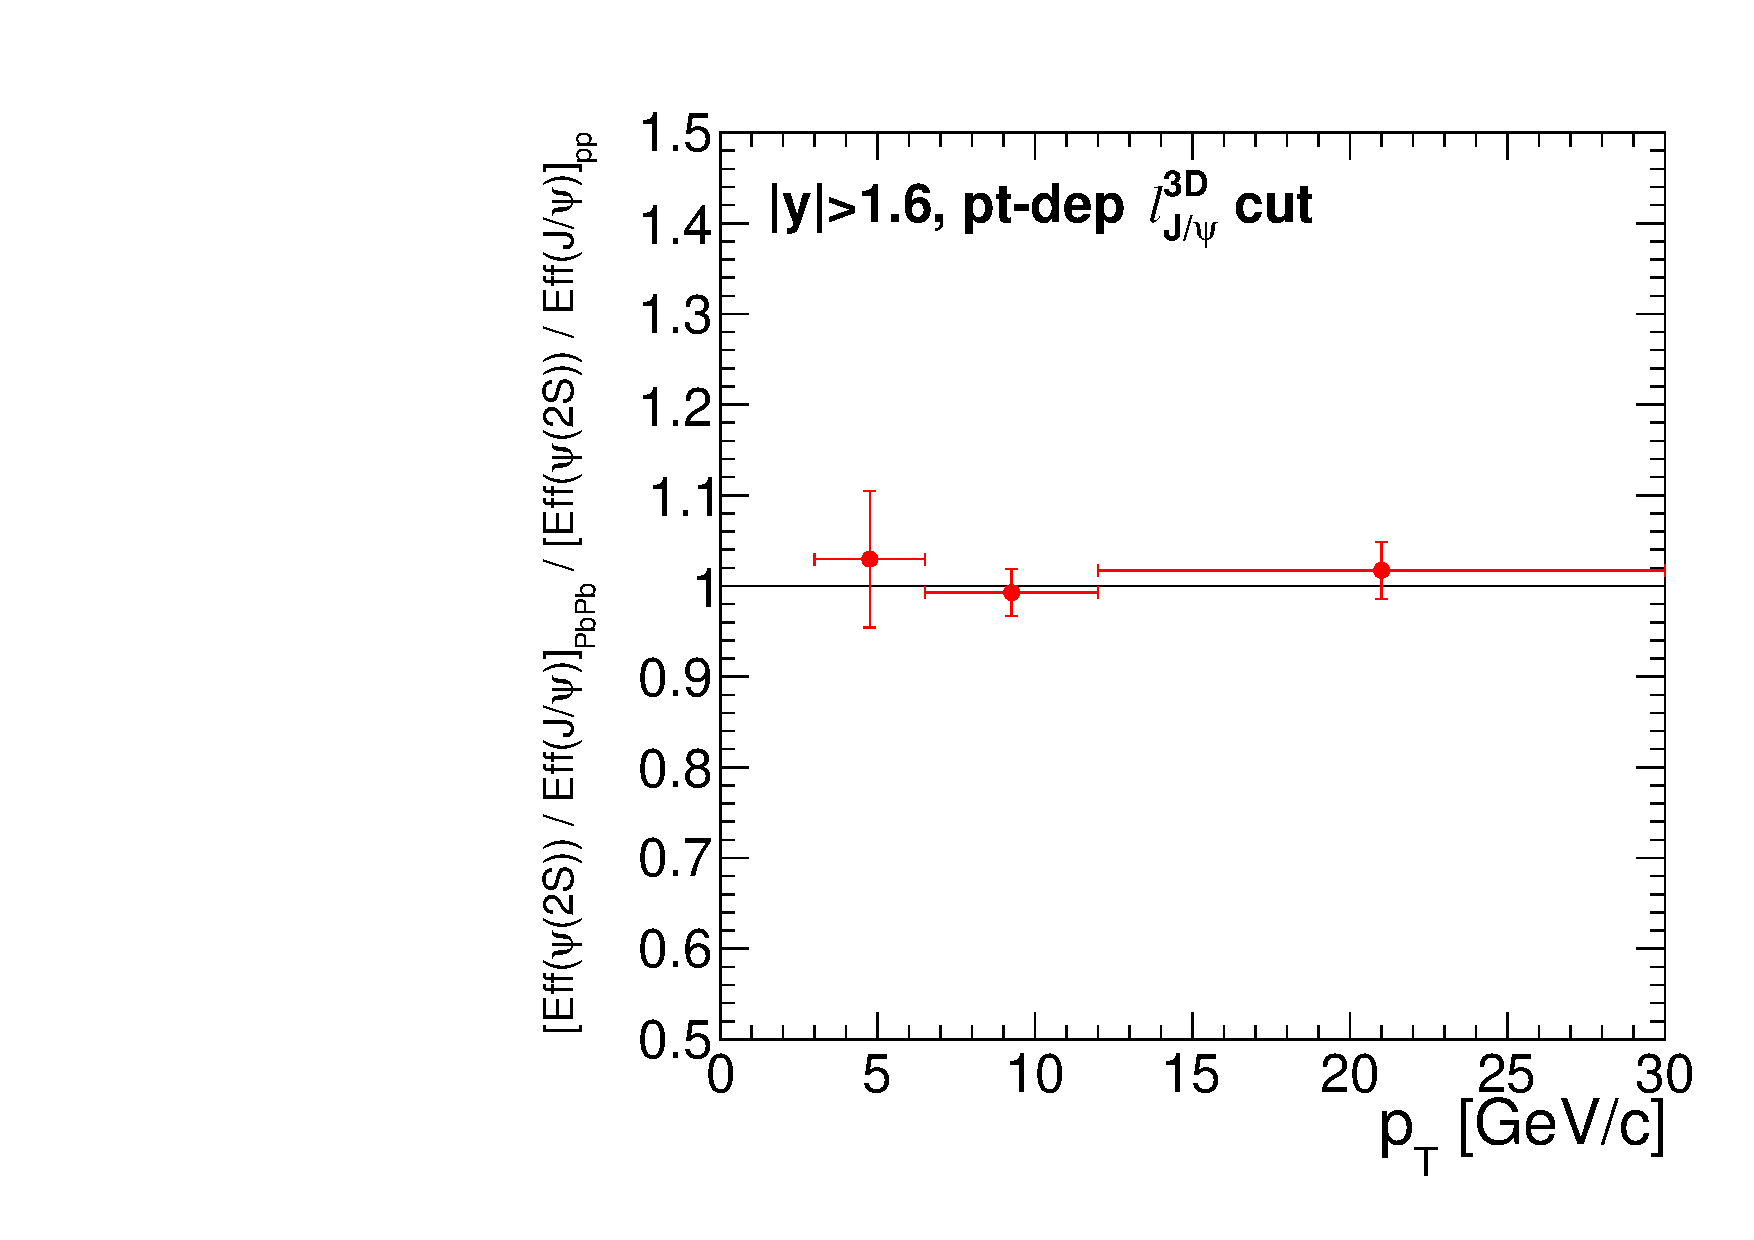
\includegraphics[width=0.45\textwidth]{Figures/Charmonia/Analysis/SignalEfficiency/DoubleRatio/doubleratio_pt_fwd_ptdepcut_.pdf}\\
 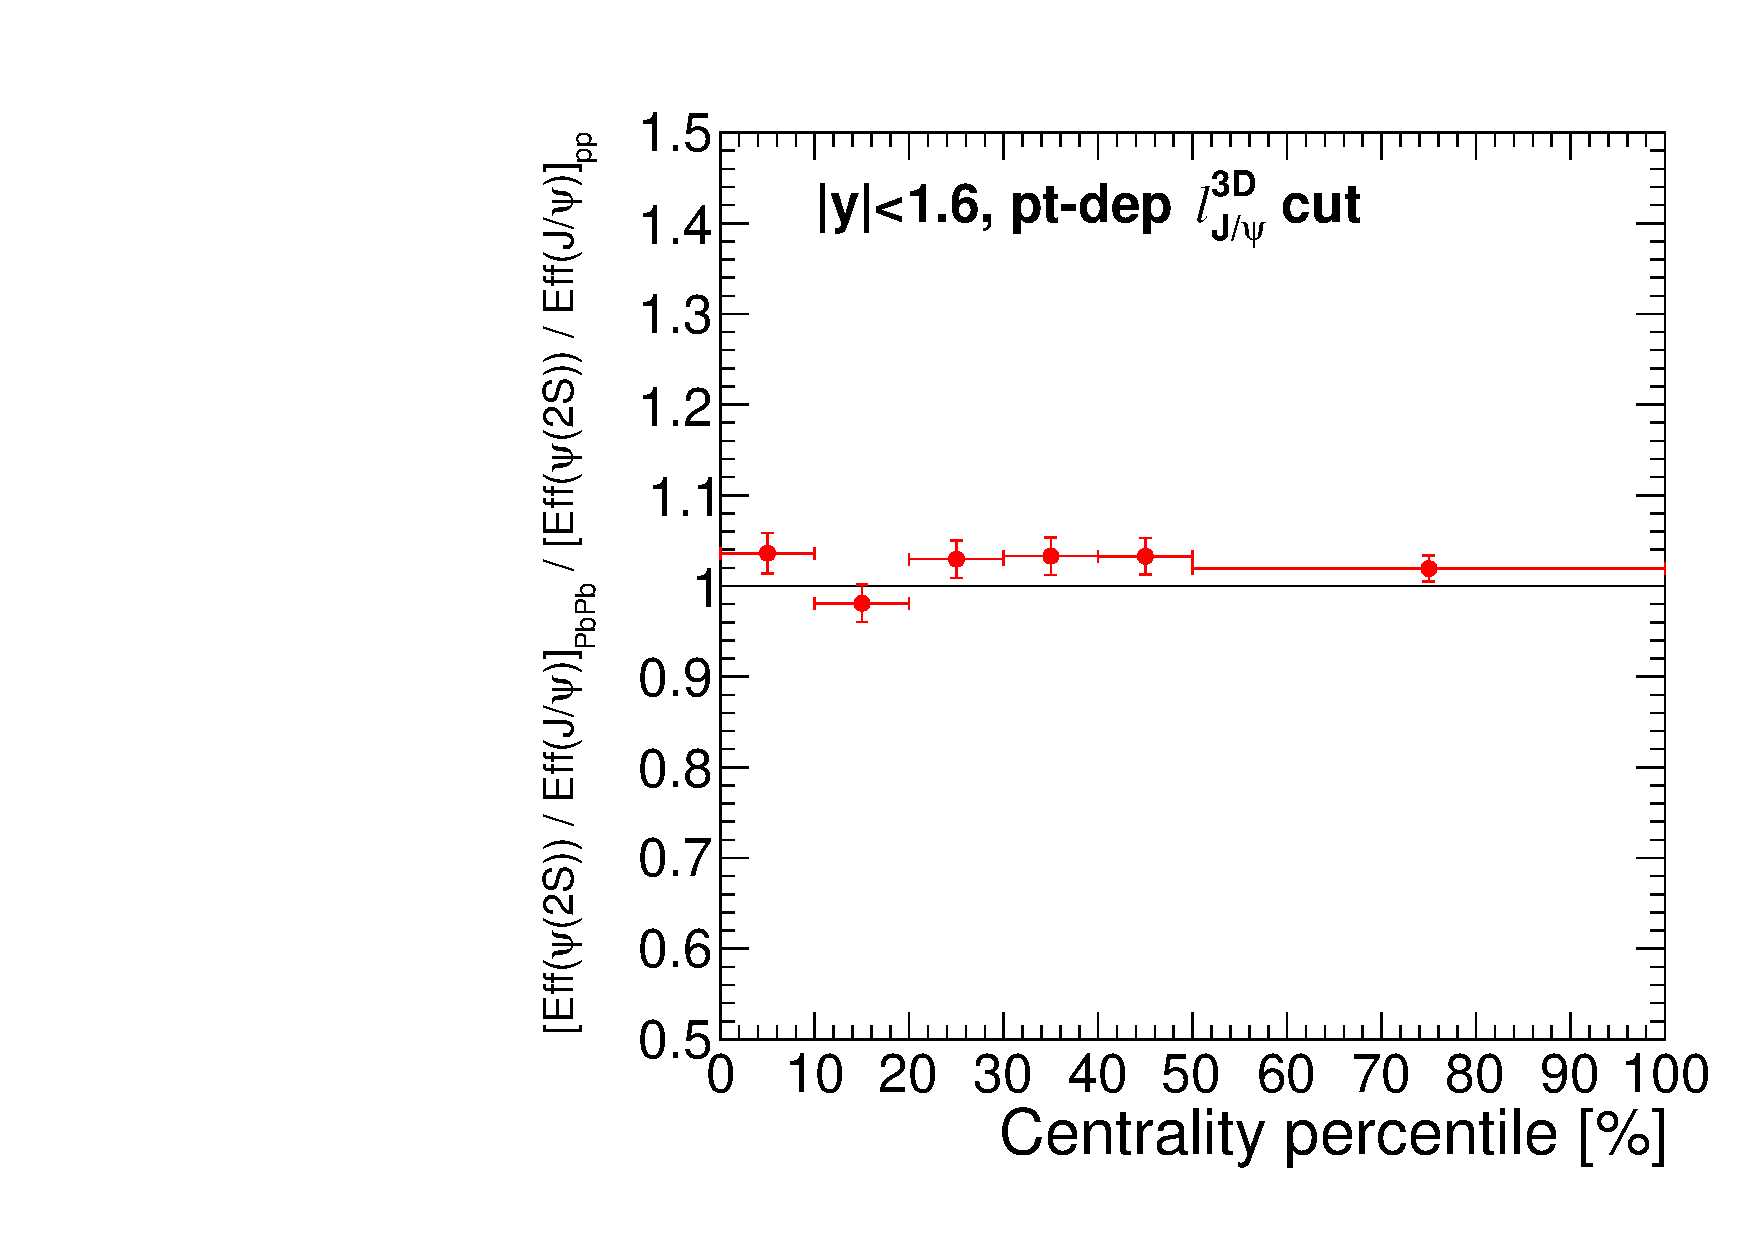
\includegraphics[width=0.45\textwidth]{Figures/Charmonia/Analysis/SignalEfficiency/DoubleRatio/doubleratio_cent_mid_ptdepcut_.pdf}
 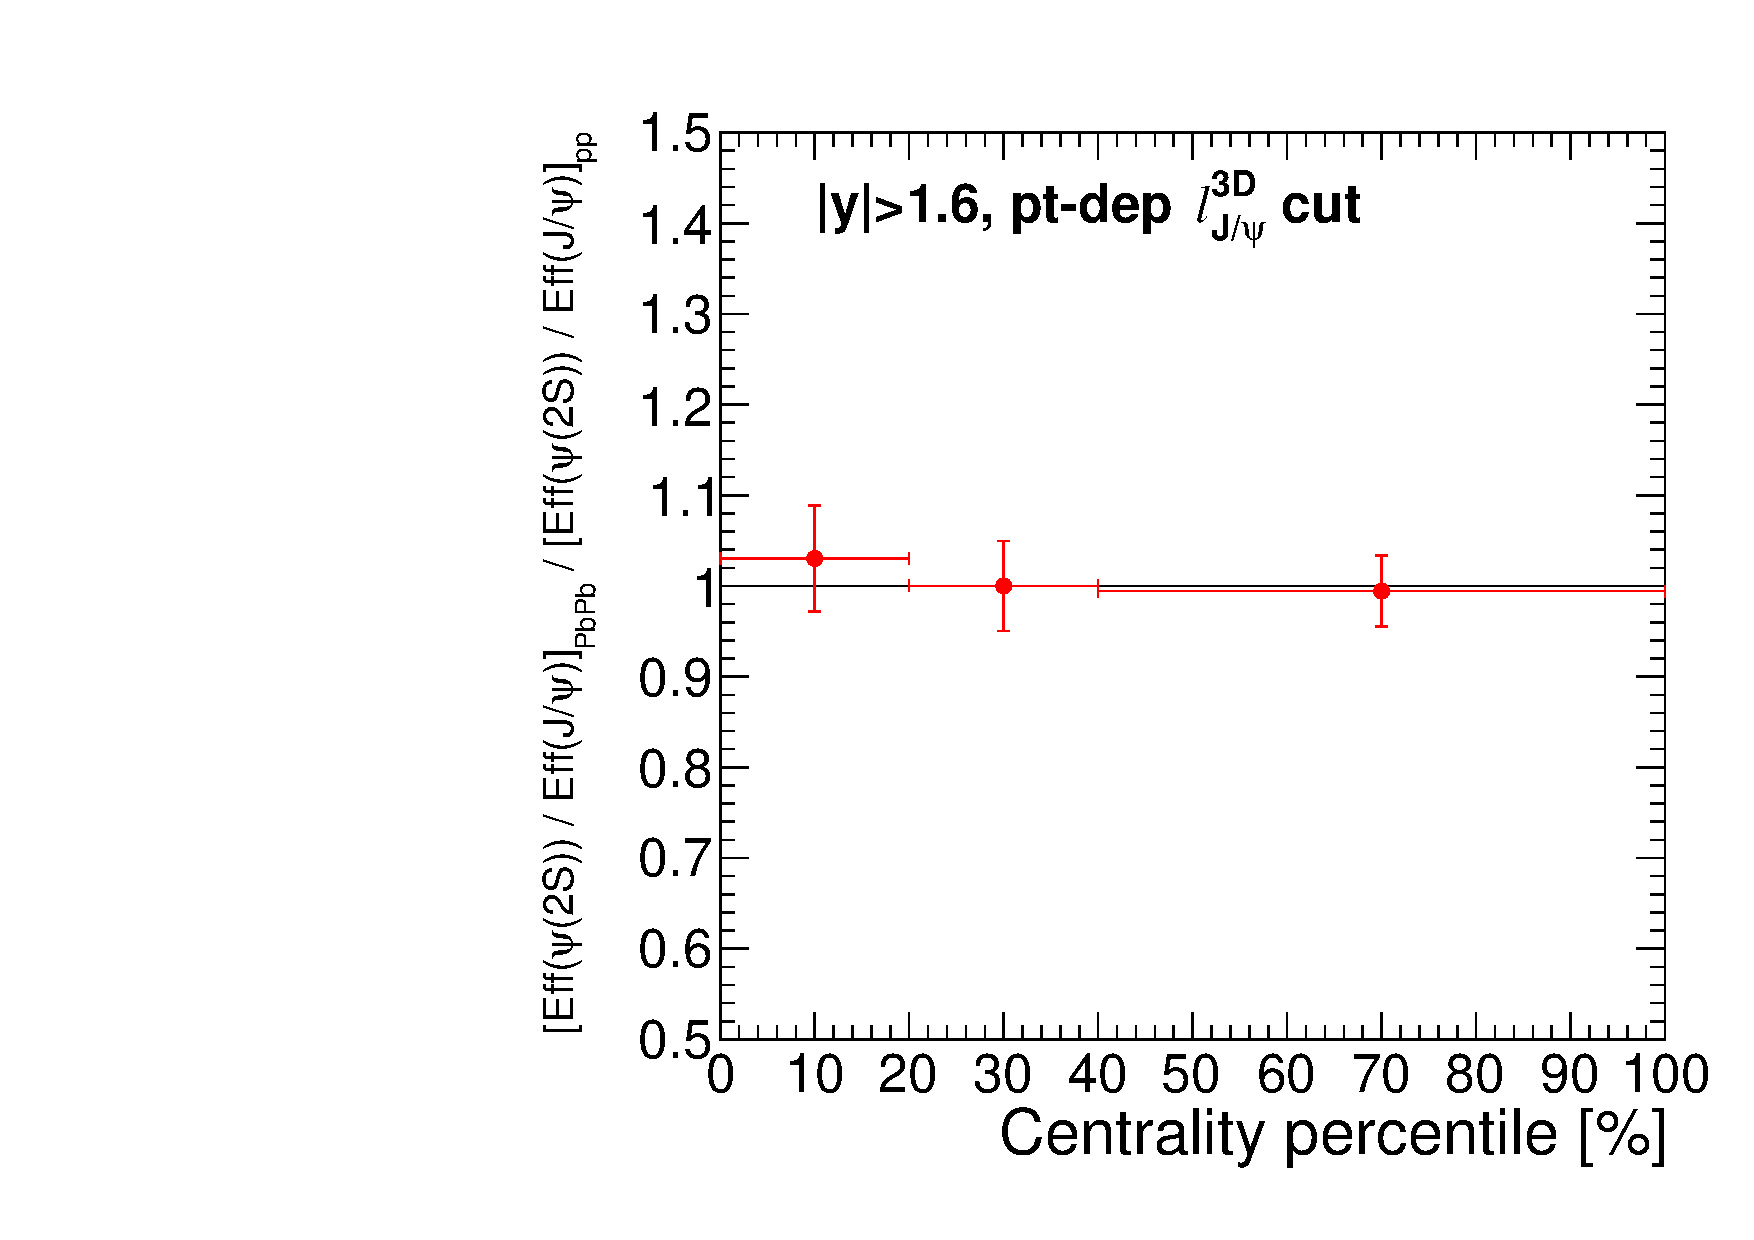
\includegraphics[width=0.45\textwidth]{Figures/Charmonia/Analysis/SignalEfficiency/DoubleRatio/doubleratio_cent_fwd_ptdepcut_.pdf}
 \caption{Double ratios of prompt charmonium efficiencies as a function of \ptMuMu (top) and centrality (bottom), in the rapidity regions: $\abs{\rapMuMu}<1.6$ (left) and $\abs{\rapMuMu}>1.6$ (right). The error bars represent statistical uncertainties.}
 \label{fig:DoubleRatioEff}
\end{figure}


% END OF SUBSECTION